% SPDX-License-Identifier: CC-BY-4.0
%
% Copyright (c) 2023 Nelson Vieira
%
% @author Nelson Vieira <nelson0.vieira@gmail.com>
% @license CC-BY-4.0 <https://creativecommons.org/licenses/by/4.0/legalcode.txt>
\section{State of the Art}

\par
This section provides an overview of the recent literature with the themes
that were found to be more relevant for this work.

\subsection{Privacy Paradox}

The use of a variety of digital devices have numerous advantages, but they
also bring with them the ubiquity of data capturing equipment, therefore,
it is understandable why the majority of online users have serious concerns
about the privacy of their personal data. However, the opinions expressed
are starkly at odds with the reality, according to Thomson et al. \cite{DarrenState}
report on the state of privacy, that just one in four European users read
the terms and conditions in their entirety prior to making an online purchase
or subscribing to a service, 59\% admitted to only quickly scanning the
terms and conditions before completing a purchase, while 14\% admitted to
never reading them at all, 30\% of the respondents would even swap their
email address to win a reward, or entry into a raffle, while 17\% would do
so to get an app and 30\% would do it for money.

This is what is called a privacy paradox, there have been multiple papers
written on this subject \cite{solove2021myth, WilliamsPrivacy, lee2021investigating, goad2021privacy, gerber2018explaining},
some papers attempt a theoretical explanation while others attempt an empirical
one. There has been very different interpretations or explanations of this
paradox, a few papers \cite{wilson2012unpacking, warshaw2015can, lee2015privacy}
apply the theoretical concept of the \textit{homo economicus} \cite{zak2008moral},
which is the representation of people as beings who constantly act in a
way that is logical and self-interested, not worrying about morality or
ethics, and who do so to the best of their ability, to the context of privacy.
Individuals' decision-making processes can be greatly influenced by a variety
of cognitive biases and heuristics, and these decisions can vary greatly from
individual to individual, according to several studies on individual choice behaviour \cite{acquisti2007can, knijnenburg2013dimensionality, wakefield2013influence, flender2012type}.
According to several articles \cite{dienlin2015privacy, baek2014solving},
this paradox might be explained by the fact that some people have genuinely
experienced online privacy assaults and that most privacy views are therefore
based on heuristics or second-hand accounts. Taddicken's study \cite{taddicken2014privacy}
argues that peer pressure is the reason people have this contradictory behaviour,
Norberg et al. \cite{norberg2007privacy} explains this paradox by suggesting
that while perceived risk affects reported attitudes and behavioural intentions,
trust has a direct impact on privacy behaviour, while others \cite{flender2012type, kokolakis2017privacy}
rely on quantum theory, meaning there is indeterminacy in the decision making,
in other words, it means that an individual's decision's result can be determined
at the time of the decision and not before. Brandimarte et al. \cite{brandimarte2013misplaced}
have explored the idea that when it comes to their data privacy, users have
an \textit{illusion of control}.

This paradox has been proven to be vitiated by a number of empirical studies \cite{dienlin2015privacy, xie2019consumers, SCHWAIG20131, sannon2018privacy},
online privacy practices are founded on separate privacy mindsets and so
they are not inherently paradoxical.

\subsection{Privacy in IoT: Approaches}

There have been a number of systematic literature reviews (SLRs) \cite{Gupta2022Privacy, Kuhtreiber2022survey, sicari2015security, LinSurvey, yang2022overview, zubaydi2023leveraging}
and systematic mapping reviews \cite{porras2018security, ahmed2019aspects}
done to study privacy and security issues in IoT.

In Gupta and Ghanavati's \cite{Gupta2022Privacy} SLR, the authors review
papers with methodologies and techniques that identify privacy risks or
notify users about these risks. They divide the literature into the following
categories: `Ontological Modeling and Semantic-based Approaches', `Data-Driven
Approaches', `Source Code Analysis-based Approaches', `User Studies and
Survey-based Approaches', `Blockchain-based Approaches' and `Architectural
and Framework-based Approaches'. They then examine current literature on
these three prerequisites. The findings show that: most works concentrate
on single IoT devices when addressing privacy threats; When analysing privacy
issues, key privacy factors such as data reduction and data aggregation
are overlooked; existing studies ignored the sensitivity of the obtained
information; most useful studies did not include a diverse range of users
when assessing privacy problems; no work has been done to discover compliance
difficulties between an IoT application and different privacy rules; and
current research does not place a premium on providing individuals with real-time
privacy notices. However, this SLR has the following limitations: the authors
only chose articles and not thesis or books and from the selected papers,
only the ones written in english were considered.

% Kühtreiber et al. \cite{Kuhtreiber2022survey} conduct a survey of the frameworks
% and tools created for developers, particularly in the case of IoT, and they conclude
% that present solutions are difficult to use, only effective in specific circumstances,
% and insufficient to address the privacy problems inherent in IoT development. This
% study lacks a comprehensive gap analysis of the chosen literature and it does not
% specify the research questions that define the relevancy of the selected papers.

% Kühtreiber et al. \cite{Kuhtreiber2022survey} evaluate the frameworks and tools
% established for developers, notably in the case of IoT, and find that current
% solutions are difficult to use, only successful in limited contexts, and insufficient
% to handle the privacy issues inherent in IoT development. This study lacks a detailed
% gap analysis of the selected literature, as well as the research questions that
% characterize the relevance of the selected publications.

Kühtreiber et al. \cite{Kuhtreiber2022survey} evaluate the frameworks and
tools established for developers, specifically in the case of IoT, and find
that current solutions are difficult to use, only successful in limited
scenarios, and insufficient to handle the privacy problems inherent in IoT
development. This study lacks a comprehensive gap review of the chosen
literature, along with research questions (RQs) establishing the significance
of the articles chosen.

% Sicari et al. \cite{sicari2015security} conduct an analysis of recent studies and
% active initiatives that emphasize IoT privacy and security solutions. They begin
% by outlining the needs for IoT privacy and security, including access control,
% confidentiality, and authentication. They then review the literature that already
% exists in relation to these three needs. They concluded that IoT privacy concerns
% are only partially investigated and need further attention. The study, however,
% has its shortcomings, the analysis of prior research focuses primarily on security
% needs and leaves out privacy considerations, they don't perform a thorough gap
% analysis on the publications that were examined, and they don't provide a thorough
% summary of the future research topics in the field of IoT privacy that need more
% attention.

% Sicari et al. \cite{sicari2015security} examine current research and ongoing activities
% that focus on IoT privacy and security solutions. They start by stating the
% requirements for IoT privacy and security, such as access control, confidentiality,
% and authentication. They next go over the existing literature in connection to these
% three needs. They came to the conclusion that IoT privacy risks have only been
% partially examined and require more attention. The study, however, has flaws: the
% analysis of prior research focuses primarily on security needs and ignores privacy
% considerations; they do not perform a thorough gap analysis on the publications
% examined; and they do not provide a comprehensive summary of future research topics
% in the field of IoT privacy that require more attention.

Sicari et al. \cite{sicari2015security} examine current research and ongoing
activities that focus on IoT privacy and security solutions. The authors
start by describing the requirements for IoT privacy and security, such
as access control, confidentiality, and authentication. The authors then
conduct a literature study in connection to these three needs. The authors
came to the conclusion that IoT privacy issues have only been partially
examined and that further attention is required. The study does, however, have
some shortcomings: the prior research analysis focuses primarily on security
requirements while ignoring privacy considerations; the authors do not conduct
a thorough gap analysis on the publications examined; and they do not provide
a comprehensive summary of future research topics in the area of IoT privacy
that require more attention.

Lin et al. \cite{LinSurvey} undertake a literature review to identify security
and privacy vulnerabilities in the three IoT architecture layers: network,
perception, and application. The authors describe the first six fundamental
security properties for these tiers as confidentiality, integrity, availability,
identification and authentication, privacy, and trust. Then, the authors
look at a variety of security threats for each of the three stages. The
authors wrap up by giving a succinct summary of many privacy-preserving
data techniques, including the stages of data collection, data aggregation,
and data analysis. The authors do, however, largely focus on the IoT's security
components and consider privacy to be one of the most crucial security aspects,
rather than viewing privacy as a distinct concern. Despite this, the authors
devote a portion of the paper to privacy and the majority of what they address
concerns security.

Yang's study \cite{yang2022overview} examines the literature from the perspective
of IoT phases, such as data collection, transmission, and storage, or in other
words, perception, network and application layers. In these phases the author explores
security protocols at the physical layer, network solutions, and data storage and
sharing approaches. There is a balance of security approaches or solutions and
non-security related approaches discussed, besides the mentioned security protocols,
the author proposes a software-defined network, for the network layer, that enables
a global view of the network which helps to identify malicious traffic patterns. The
author also suggest the use of differential privacy, privacy-preserving data mining,
blockchain or holochain for the application layer. The author presents a high-level
overview of privacy issues and as a result does not offer a comprehensive analysis of
the various approaches or make many suggestions for future study directions.

In Zubaydi et al. \cite{zubaydi2023leveraging}, different works that address the
integration of blockchain technology that aim to tackle various aspects of privacy
are analysed. This SLR has an overview of the IoT architecture, the various blockchain
types and algorithms and IoT challenges. The authors provide an overview of the
chosen papers and present a detailed comparison between them before analysing
the papers using several categories which include generic approaches, healthcare,
smart environments, IoT device gateway, IoT information systems, management systems
and other approaches. The authors also present a considerable number of open issues
that future works should focus on. Because this SLR is about blockchain technology,
the focus is on privacy through security. Overall this is a very in-depth SLR on the
use of blockchain technology to address privacy issues.

Based on Ziegeldorf's \cite{ziegeldorf2014privacy} analysis of the literature,
the following are the most prominent privacy concerns in IoT:

\begin{enumerate}
    \item
    The most prominent concern is \textit{identification}, which binds an
    identifier, such as a name and location, with an individual's identity,
    this also enables and aggravates other threats;
    \item
    \textit{Localization and tracking} is the threat of detecting an individual's
    locations through numerous techniques, such as GPS, internet traffic,
    or smartphone location. This threat requires \textit{identification}
    of some kind;
    \item
    In e-commerce, \textit{profiling} is often used for personalization.
    Organizations collect information about individuals in order to deduce
    their interests via association with other profiles and data sources.
    \item
    \textit{Interaction and presentation} allude to the sharing of private
    information with an unintended audience while doing so through a public
    medium. IoT applications often need extensive user interaction, it is
    expected that users of these systems will obtain information via smart
    devices in their immediate surroundings and that users will interface
    with systems in creative, natural ways. However, many of those modes
    of communication and presentation are already available to the broader
    public, making them apparent to anybody around. When personal information
    is transferred between a system and its user, privacy is breached.
    \item
    \textit{Lifecycle transitions} occur when an IoT device is sold, utilized
    by its owner and eventually disposed of. There may be an expectation
    that the object deletes all information, yet smart devices frequently
    keep massive volumes of data about their own past throughout their entire
    existence. This might contain personal images and videos, which are
    not always erased following ownership transfer.
    \item
    \textit{Inventory attacks} involve unauthorized entry and the acquisition
    of information about the presence and characteristics of personal things.
    Malicious users might use inventory data to profile the property and
    break in.
    \item
    \textit{Linkage} is the process of connecting disparate systems, when
    systems are connecting different data sources, there is a higher danger
    of unauthorized access and data leakage.
\end{enumerate}

Another concept worth analysing is differential privacy (DP) which relates more
closely to the survey that will be conducted but also to the general
collection and analysis of user data by applications and systems.

\subsection{Differential Privacy}

The notion of differential privacy, according to Michael Kearns \cite{kearns2019ethical},
is based on three important principles. The first being that ``differential
privacy requires that adding or removing the data record of a single individual
not change the probability of any outcome by much''. The second principle
being that ``no outside observer can learn very much about any individual
because of that person's specific data''. And the third important principle
being that ``for every individual in the dataset, and for any observer no
matter what their initial beliefs about the world were, after observing
the output of a differentially private computation, their posterior belief
about anything is close to what it would have been had they observed the
output of the same computation run without the individual's data''.

DP has the potential to significantly increase individual
privacy protection, by purposefully adding noise into a dataset, it gives
plausible deniability to any individual who may have had their data exploited
while still being able to calculate statistics with relatively high precision.
Although algorithms that deal with notions of fairness, ethics, and privacy
are hard to implement because of the subjectivity of these concepts, and
DP algorithms are no exception, they can still help in
regards to tackling technology's intrinsic ethical and moral issues.

Zhao and Chen \cite{ZhaoSurvey} conduct a SLR on DP for
unstructured data. The authors present DP methods for
sensitive content in image, audio, video, and text data. They compare the
various methods and perform utility analyses for each method, highlighting
the benefits and drawbacks of each, the utility loss is measured in experimental
evaluations between the actual data and its obfuscated variant. They come
to the conclusion that DP as well as its variations give
stringent privacy protections for unstructured data against attackers with
unpredictable background knowledge. They also suggest potential future study
subjects that have yet to be investigated.

Integrating federated learning and local differential privacy is proposed
by Zhao et al. \cite{zhao2020local} to facilitate crowdsourcing applications to
achieve the machine learning model while avoiding privacy threats and reducing
communication costs. The authors provide four mechanisms depending on the
privacy budget that is wanted. Based on experimental results of real-world
datasets, the suggested mechanisms provide stronger privacy protection when
compared to other comparable mechanisms; nevertheless, further testing is
required to establish the validity of these mechanisms on production systems.
No future research subjects are provided, only the intention of applying
these mechanisms to deep neural networks.

Similar to differential privacy, there exists different algorithms that aim to
preserve privacy such as Google's box blurring algorithm \cite{FromeLarge}
that is used in the Google Map's street view, Microsoft's Visor \cite{poddar2020visor}
which is a video-analytics-as-a-service tool and Shokri and Shmatikov's
\cite{ShokriPrivacy} system for collaborative deep learning, however, in
general, these algorithms struggle with high computational cost, internal
attacks, or non-provable privacy.

\subsection{Proposed Solutions}

\par This section list eight solutions that emerged from the structured
literature review to improve the gap between privacy and security concepts
among systems and users.

\subsubsection{User Awareness}

Although individuals have a certain expectation of privacy when using IoT
devices, privacy preferences are complex, as noted by \cite{naeini2017privacy},
some individuals value some aspects more than others. There are studies
on privacy in IoT but not many focus on user privacy awareness or
privacy literacy.

Koohang et al. \cite{koohang2022internet} propose a research model with five constructs, these being:
IoT awareness, users' IoT privacy knowledge, users' IoT security knowledge,
users' IoT Trust, and continued intention to use IoT.

An interactive theater experience was developed by Skirpan et al. \cite{SkirpanPrivacy}
as a case study of an innovative approach to gather user awareness about their
online behavior with regard to privacy. This was created to try to prove
that a simulated experience with a credible privacy problem may encourage
people to take action before actually encountering a catastrophe. The plot
of the play consist in a fledgling tech company that unveiled its revolutionary
AI technology while dealing with a company whistleblower and an untimely
zero-day hack on their system. The public is able to interact with the actors
and influence how the story plays out. Audiences and actors were given the
chance to try on roles, behaviors, and opinions that they would not normally
have access to in ordinary life. The authors had interviews and surveys
done after the plays with audience members however they only did interviews
halfway through production and only a small fraction of the audience actually
participated in this data collection, they also noted that after contacting
people months after the interviews that they did not really changed their
behaviour regarding their privacy rights.

\subsubsection{Legislation}

Some papers seek to improve legislation \cite{WEBER2015618, FabianoInternet}
because otherwise, in their view, privacy rights won't be respected if they
are not enforceable legally, they defend that without the express agreement
of the individual concerned, private information obtained by IoT devices
must not be retained or processed in any form, and necessary procedures
must be taken to guarantee that the data collected is not that of an unrelated
individual. But better protection laws for the user would also create opposition
from most companies that want to extract as much private data from their
users without (m)any restrictions in order to increase their profit margins.

\subsubsection{Privacy through Security}

Sun et al. \cite{SunSecure} design a lightweight communication strategy
for a remote-control system, employing two types of Virtual-Spaces to achieve
the aim of identity announcement and data exchange. They constructed a prototype
system of the scheme and tested it on the Freenet, demonstrating that the
method can effectively resist the influence of flow analysis on communication
anonymity while preserving communication data security.

\subsubsection{Architecture / Frameworks}

Antunes et al. \cite{AntunesFederated} do a SLR on federated learning in
the area of healthcare and make an architecture proposal. The procedure
known as federated learning allows for the distributed training of machine
learning models using remotely hosted datasets without the requirement to
gather and hence jeopardize data. The fundamental goal of the proposed architecture is
to allow healthcare institutions that have access to sensitive medical information
to use it in distributed data analysis and machine learning research while
ensuring patient confidentiality. Because information transmitted among
institutions need confidentiality guarantees for learning model parameters
and analysis results, the architecture can adopt a number of ways based on
a zero-trust security paradigm \cite{ChenSecurity}. Furthermore, the institutions
develop a learning algorithm verification system that can store and disseminate
manifestos, as well as engage in distributed analytic procedures that need
unanimous agreement from all participants. This study also demonstrates
that previous literature implies that homomorphic encryption and differential
privacy are effective approaches for preventing data breaches without incurring
prohibitively high computing costs.

Opara et al. \cite{opara2022framework} present a system for spotting possible
problems with privacy or security regulations in the early stages of development,
this approach is intended at developers. The paper proposes a domain-specific
ontology for modelling IoT security and privacy policies, a notation for
representing and validating IoT security and privacy policies, a set of
guidelines and rules for detecting IoT policy errors, and a tool for visually
modelling and capturing IoT security policies and discovering policy problems.
Although the framework that is presented is theoretically promising it has
not been tested in a real environment so the effectiveness can't yet be
measured. The authors also do not compare their proposal with others already
available.

A Privacy by Design (PbD) framework is proposed by Perera et al. \cite{perera2020designing}
to assist software developers in incorporating concerns about data privacy
into the design of IoT applications. The proposed framework consists in
a set of guidelines. The authors conducted two studies, one interview based
in person and the other online, the first study was done with software engineers with
various levels of experience and the second was done with master's students.
The authors note that developers do not have
a privacy mindset, meaning they
do not regard privacy as an primary aspect of the application design, giving
more importance to other aspects like functionality or security. They also
mentioned that using this framework must be context-based, since it may be
difficult and prone to over-analysis by engineers. When citing related
works, they state that various PbD frameworks exist but none are dedicated
to IoT, which is incorrect as evidenced by other works \cite{o2017privacy, cavoukian2016embedding},
with \cite{alkhariji2023semantics, aljeraisy2021privacy} being more recent
examples. It is true, however, that there are relatively few IoT PbD frameworks.

There exists frameworks like the NIST Cybersecurity Framework \cite{barrett2018framework},
published by the National Institute of Standards and Technology (NIST),
which includes a number of recommendations for reducing organizational
cybersecurity risks. Although this framework is primarily focused on
security, it can also be used to reduce privacy threats.
ISO/IEC 27400:2022 \cite{iso2022cybersecurity}, developed by the International
Organization for Standardization (ISO), is a standard that provides
guidelines on risks, principles and safeguards for the security and
privacy of IoT systems. In addition, ISO has produced about 208 privacy-related
standards \cite{iso2023privacysearch}, some of which have been published
and others of which are currently in development. This is a small number
when compared to the roughly 1305 security-related standards \cite{iso2023securitysearch},
but there may be some overlap between these standards. Even those ISO privacy
based standards have a good amount of intersection with security related
guidelines.

\subsubsection{Blockchain}

Blockchain is an option to guarantee privacy in IoT because of zero-knowledge
proofs\cite{sun2021survey}, ring signatures \cite{mercer2016privacy} and mixing \cite{stone2021trustless}
among other techniques \cite{zhang2019security}.

A zero-knowledge proof is a cryptographic technique that enables one party
to demonstrate to another that a certain statement is true without disclosing
any information other than the validity of that statement. Completeness, soundness,
and zero-knowledge are the three requirements that must be satisfied by a
zero-knowledge proof method. Completeness states that if a
statement is genuine, an honest party will be convinced of it by another honest
party. Soundness indicates that a nefarious party should only have a small chance
of convincing an honest party that a statement is true. Zero-knowledge states
that the method must only tell one party whether or not the other party is
disclosing the truth.

Ring signatures create a single, recognizable signature that is used to sign
a transaction by combining a number of partial digital signatures from diverse
users. This group, known as the ring, can be chosen at random from the outputs
that other users have made to the blockchain. A ring signature has the security
property that it should be computationally expensive to determine which
of the group's members' keys was used to produce the signature, this is because
it obfuscates the input side of a transaction. A user's anonymity cannot
be taken away from their signature, and any group of users can act as a signing
group automatically.

Mixing is the process of blending possibly traceable digital assets
with others to obscure the original assets' sources. This is frequently done
by pooling source assets from different inputs for a long period and at random
intervals, then spitting them back out to destination addresses. Since they
are all packed together and then delivered at random intervals, it is very
difficult to pinpoint particular assets. Due to the fact that cryptocurrencies
provide a public record of every transaction, mixers have been developed
to improve cryptocurrency privacy. Because of their emphasis on secrecy,
mixers have been used to launder money using cryptocurrency.

Zhang et al. \cite{zhang2019security} outline some disadvantages concerning
these techniques. For example, the authors assert that zero-knowledge proofs
are less efficient than other techniques, that ring signatures cannot reveal
the identity of the signer in the event of a dispute, and that centralized
services run an increased risk of leaking users' personal information when
it comes to mixing.

Yu et al. \cite{yu2018blockchain} discuss various implementations of blockchain
that provide privacy through security, based on different categories like
data integrity, data sharing and authentication and access control, most
implementations proposed use a peer-to-peer network based on the Ethereum
platform, with the exception being using any consortium or private blockchain,
consortium meaning a blockchain where consensus is managed by a pre-selected set
of nodes and private meaning access permission and read/write authority are
tightly controlled. The authors use privacy as a proxy for security, they also
do not discuss the weak and strong points of each implementation or make any
comparison, they also do not provide further research questions.

Ali et al. \cite{AliIoT} suggest a software stack that combines peer-to-peer
file sharing with blockchain smart contracts to offer IoT users control
over their data and do away with the necessity for centralized IoT data
management. Blockchain smart contracts are used in the proposed `modular
consortium' architecture to regulate access while establishing responsibility
for both data owners and other parties that users grant access to.

\subsubsection{Privacy Assistants}

There exists a number of privacy assistants in the market. Privacy assistants
have the objective of giving the user flexibility in choosing the preferred
privacy options in available applications, most are used in smartphones,
very few are made for devices in the IoT.

The Carnegie Mellon University CyLab, which is the university's security
and privacy research institute, started developing in 2019 an IoT Infrastructure
that intended to be free of privacy leaks and software covered by their
Secure and Private IoT Initiative 2019, this project would fall under
their main research theme of Trust. In this project they started the design
of a Personalized Privacy Assistant (PPA) \cite{ColnagoInforming}, this
would involve the use of semi-structured interviews with 17 participants
to examine user perceptions of three hypothetical PPA implementations,
each of which is potentially more autonomous, while outlining the advantages
and disadvantages of each implementation. The interviews were divided into
three sections: exploratory, anchoring and the PPA; While the exploratory
phase's purpose was to learn about participants' attitudes and understanding
of IoT, the anchoring phase aimed to normalize participants' basic understanding
of how IoT functions. In order to get people to think about potential privacy
concerns towards the end of the anchoring section, the authors asked participants
about their opinions on data privacy. In the PPA section, it was proposed
the idea of a PPA for IoT as a potential future project. The authors clarified
that the PPA could distinguish between active data requests such as a gadget
asking biometric information from the user's health tracker and passive
data collection such as a smart device with a microphone that could record
people's utterances while they were nearby. The Notification, Recommendation,
and Auto implementations of an IoT PPA were the three that the authors and
attendees discussed. Notification PPAs can determine which adjacent devices
are requesting data and alert users to those devices' presence and requests
so that users can approve or reject each request. Building on notification
PPAs, recommendation PPAs offer advice to individuals on how to share their data
based on their preferences. The user's data sharing decisions would be made
by auto PPAs. This would lessen the cognitive load on individuals but also
take away their ability to influence the process. They found that the participants'
attitudes regarding the various implementations were generally favourable,
although they also voiced worries, which varied depending on the degree
of automation. Given the divergent motivations of participants some desired
increased control, while others wished to avoid being overtaken by notifications
and the lack of agreement regarding the optimal PPA implementation.

After the design phase, the institute implemented a privacy assistant (PA) \cite{FengDesign},
the authors called it IoT Assistant. Because the predominant approach of
"notice and choice" for data privacy protection, they decided the PA would
also fall into this approach, but because many systems implement notice
as a form of consent, without sometimes offering choices to the end user,
they also wanted this work to provide a conceptual framework that views
user-centred privacy choice as well as a taxonomy for practitioners to
use when designing meaningful privacy choices for their systems. The authors
define meaningful privacy choices as ``the capabilities provided by digital
systems for users to control different data practices over their personal
data'', They extend the notion of privacy choices with five facets: effectiveness
(the opportunity to establish privacy preferences that precisely and completely
match the data collection and use methods that a user is okay with), efficiency
(the capacity to specify these options with the least amount of effort and
time), user awareness (where significant privacy options should be prominently
and clearly communicated to users), comprehensiveness (users should understand
their options, how they affect the gathering and potential use of their
data, as well as what conclusions might be drawn from this data and the
potential repercussions of these conclusions) and neutrality (meaningful
privacy decisions should not be subject to manipulation or bias). The IoT
Assistant offers four privacy settings, giving end users a variety of alternatives
to better suit their varied privacy preferences and as a result, privacy
options are more effective in the IoT environment. The IoT Assistant acts
as a centralized privacy choice platform by implementing various privacy
options, allowing individuals to more effectively govern their data privacy
in IoT. The three IoT system discovery modes that the IoT Assistant supports
are QR codes, push notifications, and location-based map interfaces. These
discovery tools are probably going to make users more aware of the installed
IoT devices and the privacy options they have. Additionally, the united
viewpoint of the integrated notification and option in the the IoT Assistant
gives succinct yet thorough information regarding IoT data practices to
help users better understand the implications of their privacy choices.
Additionally, the authors work to implement the integrated notice and option
in the IoT Assistant without bias or framing, attempting to offer individuals
a neutral space to execute their privacy choices. Although the authors view
the IoT Assistant as a significant step towards ``meaningful privacy options''
in IoT, this assistant still has many problems, such as the fact that it
is still in its early stages of development and that there hasn't been much
growth given that it was created in 2020 and we are in 2023. Maybe the main
reason this application was not able to be developed further is that the
application itself serves to show the user the data that is already in the
IoT infrastructure that was created before, and as such it is not capable
of identifying new IoT devices without the end users themselves create on
the infrastructure's main webpage \cite{DasPersonalized} a new entry for
the device in question that the user wants to interact with. Another reason
that cripples this application as well as others that seek to provide better
privacy in IoT systems is that many systems do not offer any type of privacy
choices to the end user or to other users that are not the intended end
users but the devices are still collecting data about.

The IoT infrastructure that was developed \cite{DasPersonalized} is built
on an open, distributed design that allows for the deployment and management
of IoT resources to be carried out by any number of actors. Part of this
infrastructure is the Internet of Things Resource Registry, it is a web
platform that enables resource owners to declare not only the place where
a resource is deployed but also data practices like the reason(s) for a
particular data collecting process, the level of detail in the data being
gathered, retention, the recipients of the data, and more. Additionally,
it discloses any user-configurable privacy settings that might be connected
to a particular resource.

\subsubsection{Sniffers}

IoT sniffers are usually used to detect problems in the networks, they rarely
are used to provide privacy for the users.

The LTEye project \cite{KumarLTE} is an open platform that provides granular
temporal and spatial analytics on the performance of LTE radios without access
to private user data or provider assistance. Despite the presence of multipath,
LTEye uses a revolutionary extension of synthetic aperture radar to communication
signals in order to precisely pinpoint mobile users.

\subsubsection{Other Proposals}

Zhu et al. \cite{ZhuIntegrating} present a hybrid sensor system that safeguards
privacy while also monitoring parking availability. The authors merged IoT
sensing with crowdsensing and enhanced it with privacy-preserving methods.
The authors employed physical hazy filters to mask IoT sensors in IoT sensing,
and a cryptographic technique based on cryptographic commitments, zero-knowledge
proofs, and anonymous credentials in crowdsensing. In addition, they used
crowdsourcing to create a machine learning model for parking recognition
in the presence of foggy filters. Their paper included proof-of-concept
prototypes such as a Raspberry Pi system and a mobile app, as well as an
evaluation study of the machine learning model and the effects of crowdsourcing.

\subsection{Findings Analysis}

% \begin{table}[H]
%     \begin{center}
%         \begin{tabular}{r *{4}{ p{5cm} }}
%             \hline
%             Ref $\#$ & Type of approach & Pros & Cons \\
%             \hline
%             1\hspace{0.5cm} & General knowledge and attitudes towards privacy & This
%             section's goal is to ask generic questions regarding the participants awareness
%             of information privacy. \\
%             \hline
%             2\hspace{0.5cm} & Disposition for sharing personal information & This
%             section is designed to elicit generic inquiries about the participants
%             willingness to provide personal information. \\
%             \hline
%             3\hspace{0.5cm} & Privacy concerns & This section strives to
%             elicit questions about potential concerns about disclosing
%             personal information. \\
%             \hline
%             4\hspace{0.5cm} & Current online habits and practices & This
%             section includes general questions with regard to working with
%             the internet in everyday activities. \\
%             \hline
%             5\hspace{0.5cm} & Profile identification & This section gathers
%             more particular questions concerning employing profiles to make
%             it more straightforward to generate tailor-made interactions. \\
%             \hline
%             6\hspace{0.5cm} & Knowledge and habits regarding the Internet
%             of Things & This section contains questions about participants'
%             usage patterns for IoT devices as well as questions that aim to
%             understand their level of literacy. \\
%             \hline
%             7\hspace{0.5cm} & Demographic data & This section is for
%             gathering broad demographic information that allows
%             to characterize the participants in statistical terms. \\
%             \hline
%             8\hspace{0.5cm} & Demographic data & This section is for
%             gathering broad demographic information that allows
%             to characterize the participants in statistical terms. \\
%             \hline
%         \end{tabular}
%     \end{center}
%     \vspace{1em}
%     \caption{Summary of literature}
%     \label{table:literature_by_topics}
% \end{table}

\begin{footnotesize}
    \begin{longtable}{p{1.2cm} p{1cm} p{1.5cm} p{3.2cm} p{5cm} p{3cm}}
        \hline
        \textbf{Ref $\#$} & \textbf{Year} & \textbf{Country} & \textbf{Publication Type} & \textbf{Publisher} & \textbf{Domain(s)} \\
        \hline
        \endfirsthead
        \multicolumn{6}{@{}l}{\dots continued}\\\hline
        \textbf{Ref $\#$} & \textbf{Year} & \textbf{Country} & \textbf{Publication Type} & \textbf{Publisher} & \textbf{Domain(s)} \\
        \hline
        \endhead
        \multicolumn{6}{r@{}}{continues \ldots}\\
        \endfoot
        \endlastfoot
        % \cite{DarrenState} & 2015 & USA & Tech Report & \textbf{Norton} NortonLifeLock & Statistical analisys \\
        % \hline
        % \cite{solove2021myth} & 2021 & USA & Journal & \textbf{George Washington University} George Washington Law Review & Privacy paradox \\
        % \hline
        % \cite{WilliamsPrivacy} & 2017 & UK & Conference & \textbf{IEEE} 15th Annual Conference on Privacy, Security and Trust (PST) & Privacy paradox \\
        % \hline
        % \cite{lee2021investigating} & 2021 & South Korea & Journal & \textbf{MDPI} Sustainability & Privacy paradox \\
        % \hline
        % \cite{goad2021privacy} & 2021 & Australia & Journal & \textbf{Elsevier} Information \& Management & Privacy paradox \\
        % \hline
        % \cite{gerber2018explaining} & 2018 & USA & Journal & \textbf{Elsevier} Computers \& security & Privacy paradox \\
        % \hline
        % \cite{wilson2012unpacking} & 2012 & USA & Conference & \textbf{AIS} 33rd International Conference on Information Systems & Privacy paradox \\
        % \hline
        % \cite{warshaw2015can} & 2015 & USA & Conference & \textbf{ACM} Proceedings of the 33rd Annual ACM Conference on Human Factors in Computing Systems & Privacy paradox \\
        % \hline
        % \cite{lee2015privacy} & 2015 & South Korea & Journal & \textbf{Elsevier} Expert Systems with Applications & Privacy paradox and healthcare \\
        % \hline
        % \cite{zak2008moral} & 2008 & USA & Book & \textbf{Princeton University Press} & Morality in economy \\
        % \hline
        % \cite{acquisti2007can} & 2007 & USA & Book & \textbf{Auerbach Publications} & Digital Privacy \\
        % \hline
        % \cite{knijnenburg2013dimensionality} & 2013 & USA & Journal & \textbf{Elsevier} International Journal of Human-Computer Studies & Privacy paradox \\
        % \hline
        % \cite{wakefield2013influence} & 2013 & USA & Journal & \textbf{Elsevier} The Journal of Strategic Information Systems & Privacy paradox \\
        % \hline
        % \cite{flender2012type} & 2012 & Germany & Conference & \textbf{Springer} International Symposium on Quantum Interaction & Privacy paradox \\
        % \hline
        \cite{dienlin2015privacy} & 2015 & Germany & Journal & \textbf{Wiley} European Journal of Social Psychology & Privacy paradox \\
        \hline
        \cite{baek2014solving} & 2014 & South Korea & Journal & \textbf{Elsevier} Computers in Human Behavior & Privacy paradox \\
        \hline
        \cite{taddicken2014privacy} & 2014 & Germany & Journal & \textbf{Oxford University Press} Journal of Computer-Mediated Communication & Privacy paradox \\
        \hline
        \cite{norberg2007privacy} & 2007 & USA & Journal & \textbf{Wiley} Journal of Consumer Affairs & Privacy paradox \\
        \hline
        \cite{kokolakis2017privacy} & 2017 & Greece & Journal & \textbf{Elsevier} Computers \& security & Privacy paradox \\
        \hline
        \cite{brandimarte2013misplaced} & 2013 & USA & Journal & \textbf{SAGE Publications} Social Psychological and Personality Science & Privacy paradox \\
        \hline
        \cite{xie2019consumers} & 2019 & USA & Journal & \textbf{Taylor \& Francis} Journal of Interactive Advertising & Privacy paradox \\
        \hline
        \cite{SCHWAIG20131} & 2013 & USA & Journal & \textbf{Elsevier} Information \& Management & Individual's online behaviour \\
        \hline
        \cite{sannon2018privacy} & 2018 & USA & Conference & \textbf{ACM} Proceedings of the 2018 CHI Conference on Human Factors in Computing Systems & Privacy paradox \\
        \hline
        \cite{Gupta2022Privacy} & 2022 & USA & Journal & \textbf{IEEE} Internet of Things Journal & Systematic Literature Review \\
        \hline
        \cite{Kuhtreiber2022survey} & 2022 & Germany & Journal & \textbf{Elsevier} Pervasive and Mobile Computing & Systematic Literature Review \\
        \hline
        \cite{sicari2015security} & 2015 & Italy & Journal & \textbf{Elsevier} Computer Networks & Systematic Literature Review \\
        \hline
        \cite{LinSurvey} & 2017 & China & Journal & \textbf{IEEE} Internet of Things Journal & Systematic Literature Review \\
        \hline
        % \cite{porras2018security} & 2018 & Finland & Conference & \textbf{AIS} Proceedings of the 51st Hawaii International Conference on System Sciences & Systematic Mapping Review \\
        % \hline
        % \cite{ahmed2019aspects} & 2019 & Czech Republic & Journal & \textbf{IEEE} Access & Systematic Mapping Review \\
        % \hline
        \cite{yang2022overview} & 2022 & Norway & Journal & \textbf{Frontiers} Frontiers in Artificial Intelligence & Systematic Literature Review \\
        \hline
        \cite{zubaydi2023leveraging} & 2022 & Hungary & Journal & \textbf{MDPI} Sensors & Systematic Literature Review \\
        \hline
        \cite{ziegeldorf2014privacy} & 2014 & Germany & Journal & \textbf{Wiley} Security and Communication Networks & Systematic Literature Review \\
        \hline
        % \cite{kearns2019ethical} & 2019 & UK & Book & \textbf{Oxford University Press} & Privacy algorithms \\
        % \hline
        % \cite{FromeLarge} & 2009 & USA & Conference & \textbf{IEEE} International Conference on Computer Vision & Image Protection \\
        % \hline
        % \cite{poddar2020visor} & 2020 & USA & Conference & \textbf{USENIX} Proceedings of the 29th USENIX Security Symposium & Video Analytics \\
        % \hline
        % \cite{ShokriPrivacy} & 2015 & USA & Conference & \textbf{ACM} Proceedings of the 22nd ACM SIGSAC Conference on Computer and Communications Security & Machine learning \\
        % \hline
        \cite{ZhaoSurvey} & 2022 & Australia & Journal & \textbf{ACM} Computing Surveys & Differential Privacy \\
        \hline
        \cite{zhao2020local} & 2020 & Singapore & Journal & \textbf{IEEE} Internet of Things Journal & Differential Privacy, Federated Learning \\
        \hline
        \cite{SkirpanPrivacy} & 2022 & USA & Magazine & \textbf{ACM} Communications of the ACM & New ways for user awareness \\
        \hline
        \cite{WEBER2015618} & 2015 & Switzerland & Journal & \textbf{Elsevier} Computer Law \& Security Review & Legislation \\
        \hline
        \cite{FabianoInternet} & 2017 & Italy & Conference & \textbf{IEEE} International Conference on Internet of Things (iThings) and IEEE Green Computing and Communications (GreenCom) and IEEE Cyber, Physical and Social Computing (CPSCom) and IEEE Smart Data (SmartData) & Legislation \\
        \hline
        \cite{SunSecure} & 2022 & China & Journal & \textbf{ACM} Transactions on Sensor Networks & Peer to peer network \\
        \hline
        \cite{AntunesFederated} & 2022 & Brazil & Journal & \textbf{ACM} Transactions on Intelligent Systems and Technology & Healthcare \\
        \hline
        % \cite{ChenSecurity} & 2021 & China & Journal & \textbf{IEEE} Internet of Things Journal & Healthcare \\
        % \hline
        \cite{opara2022framework} & 2022 & USA & Conference & \textbf{ACM} Proceedings of the 37th ACM/SIGAPP Symposium on Applied Computing & Framework \\
        \hline
        \cite{perera2020designing} & 2019 & UK & Journal & \textbf{Elsevier} Information Sciences & Framework \\
        \hline
        \cite{barrett2018framework} & 2018 & USA & Tech Report & \textbf{NIST} Cybersecurity Framework & Framework \\
        \hline
        \cite{iso2022cybersecurity} & 2022 & USA & Tech Report & \textbf{ISO} IT Security & IT Standards \\
        \hline
        % \cite{mercer2016privacy} & 2016 & UK & Master's Report & \textbf{University College London} & Blockchain \\
        % \hline
        \cite{zhang2019security} & 2019 & China & Journal & \textbf{ACM} Computing Surveys & Blockchain \\
        \hline
        \cite{yu2018blockchain} & 2018 & China & Journal & \textbf{IEEE} Wireless Communications & Blockchain \\
        \hline
        \cite{AliIoT} & 2017 & Italy & Conference & \textbf{ACM} Proceedings of the Seventh International Conference on the Internet of Things & Blockchain \\
        \hline
        \cite{ColnagoInforming} & 2020 & USA & Conference & \textbf{ACM} Proceedings of the 2020 CHI Conference on Human Factors in Computing Systems & Privacy Assistant \\
        \hline
        \cite{FengDesign} & 2021 & USA & Conference & \textbf{ACM} Proceedings of the 2021 CHI Conference on Human Factors in Computing Systems & Privacy Assistant \\
        \hline
        \cite{DasPersonalized} & 2018 & USA & Journal & \textbf{IEEE} Pervasive Computing & Privacy Assistant \\
        \hline
        \cite{KumarLTE} & 2014 & USA & Conference & \textbf{ACM} Proceedings of the 2014 ACM Conference on SIGCOMM & Sniffer \\
        \hline
        \cite{ZhuIntegrating} & 2022 & Australia & Journal & \textbf{ACM} Transactions on Internet of Things & Smart City \\
        \hline
        \caption{Information of papers}
        \label{table:literature_overview}
    \end{longtable}
\end{footnotesize}

\begin{table}[H]
    \begin{center}
        \begin{tabular}{p{1.2cm} p{4cm} p{5cm} p{5cm}}
            \hline
            \textbf{Ref $\#$} & \textbf{Type of Approach} & \textbf{Pros} & \textbf{Cons} \\
            \hline
            \cite{dienlin2015privacy} & Privacy paradox & Pros & Cons \\
            \hline
            \cite{baek2014solving} & Privacy paradox & Pros & Cons \\
            \hline
            \cite{taddicken2014privacy} & Privacy paradox & Pros & Cons \\
            \hline
            \cite{norberg2007privacy} & Privacy paradox & Pros & Cons \\
            \hline
            \cite{kokolakis2017privacy} & Privacy paradox & Pros & Cons \\
            \hline
            \cite{brandimarte2013misplaced} & Privacy paradox & Pros & Cons \\
            \hline
            \cite{xie2019consumers} & Privacy paradox & Pros & Cons \\
            \hline
            \cite{SCHWAIG20131} & Individual's online behaviour & Pros & Cons \\
            \hline
            \cite{sannon2018privacy} & Privacy paradox & Pros & Cons \\
            \hline
            \cite{Gupta2022Privacy} & Systematic Literature Review & Pros & Cons \\
            \hline
            \cite{Kuhtreiber2022survey} & Systematic Literature Review & Pros & Cons \\
            \hline
            \cite{sicari2015security} & Systematic Literature Review & Pros & Cons \\
            \hline
            \cite{LinSurvey} & Systematic Literature Review & Pros & Cons \\
            \hline
            \cite{yang2022overview} & Systematic Literature Review & Pros & Cons \\
            \hline
            \cite{zubaydi2023leveraging} & Systematic Literature Review & Pros & Cons \\
            \hline
            \cite{ziegeldorf2014privacy} & Systematic Literature Review & Pros & Cons \\
            \hline
            \cite{ZhaoSurvey} & Differential Privacy & Pros & Cons \\
            \hline
            \cite{zhao2020local} & Differential Privacy, Federated Learning & Pros & Cons \\
            \hline
            \cite{SkirpanPrivacy} & New ways for user awareness & Pros & Cons \\
            \hline
            \cite{WEBER2015618} & Legislation & Pros & Cons \\
            \hline
            \cite{FabianoInternet} & Legislation & Pros & Cons \\
            \hline
            \cite{SunSecure} & Peer to peer network & Pros & Cons \\
            \hline
            \cite{AntunesFederated} & Healthcare & Pros & Cons \\
            \hline
            \cite{opara2022framework} & Framework & Pros & Cons \\
            \hline
            \cite{perera2020designing} & Framework & Pros & Cons \\
            \hline
            \cite{zhang2019security} & Blockchain & Pros & Cons \\
            \hline
            \cite{yu2018blockchain} & Blockchain & Pros & Cons \\
            \hline
            \cite{AliIoT} & Blockchain & Pros & Cons \\
            \hline
            \cite{ColnagoInforming} & Privacy Assistant & Pros & Cons \\
            \hline
            \cite{FengDesign} & Privacy Assistant & Pros & Cons \\
            \hline
            \cite{DasPersonalized} & Privacy Assistant & Pros & Cons \\
            \hline
            \cite{KumarLTE} & Sniffer & Pros & Cons \\
            \hline
            \cite{ZhuIntegrating} & Smart City & Pros & Cons \\
            \hline
        \end{tabular}
    \end{center}
    \vspace{1em}
    \caption{Summary of literature}
    \label{table:literature}
\end{table}

% A summary of the literature with the pros and cons can be seen on Table \ref{table:literature}.
There are two main ways to provide privacy in IoT systems, through security
or using privacy notices, other ways like through legislation or with the
creation/usage of a framework that provides privacy fall into these two
categories. Most of the literature assumes that security and privacy are
synonyms, for example \cite{opara2022framework, FabianoInternet, SunSecure},
and so most of the proposed solutions fall under privacy through security.
The proposed solutions that use privacy notices, like \cite{FengDesign},
are implemented in a way that use other devices like smartphones that provide
the notices themselves, it is hard to provide privacy notices on the IoT
devices themselves because many of these devices do not have a screen or
the screen is too small to provide the necessary information to the user.
Because there are still no standards for implementing privacy notices, and
best practices are scattered throughout the literature, they are mostly
implemented haphazardly, little guidance is given to designers and developers
on how to make a privacy notice design that is sufficient and acceptable
for their particular system and its features. Designers may be unaware of
the numerous possibilities for creating acceptable privacy notifications
and, as a result, do not systematically explore them.

Aleisa and Renaud \cite{aleisa2016privacy} also identify security and privacy
awareness as potential solutions to privacy issues in IoT, but also identify
data minimization, hitchhiking and introspection. Data minimization entails
limiting the collecting of personal information to what is absolutely central
and retaining the data just for as long as is required to satisfy the goal
of the technology's services \cite{ojDirective281}. Hitchhiking \cite{tang2006putting}
is a method of protecting the privacy of users who divulge their location,
applications regard locations as the object of their attention. The fidelity
trade-off is removed as it is not important to know who is in a certain
location. The introspection \cite{kang2015protection} method examines Virtual
Machine (VM) actions to adequately safeguard users' private information.
Every VM's CPU status, memory contents, network information provided by the
hypervisor, and any malicious software that may be present on the VM are
all collected and analysed. The privacy of individuals is jeopardized if
an IoT device loses integrity due to a hostile assault.

\begin{figure}
    \begin{center}
        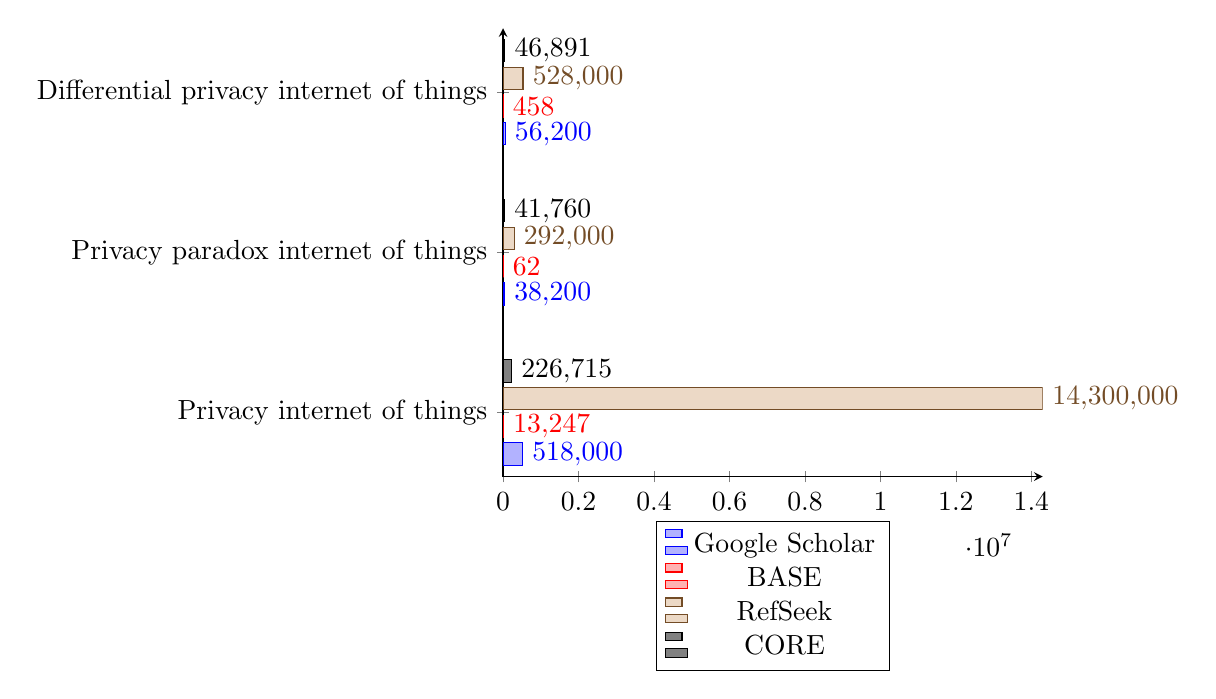
\begin{tikzpicture}
            \begin{axis}[
                xbar,
                symbolic y coords={Privacy internet of things,Privacy paradox internet of things,Differential privacy internet of things},
                bar width=8pt,
                ytick=data,
                axis x line=bottom,
                axis y line=left,
                enlarge y limits=0.2,
                nodes near coords={\pgfmathprintnumber[fixed]\pgfplotspointmeta},
                legend style={at={(0.5,-0.1)},anchor=north}
            ]
                \addplot coordinates {(518000,Privacy internet of things) (38200,Privacy paradox internet of things) (56200,Differential privacy internet of things)};
                \addlegendentry{Google Scholar}
                \addplot coordinates {(13247,Privacy internet of things) (62,Privacy paradox internet of things) (458,Differential privacy internet of things)};
                \addlegendentry{BASE}
                \addplot coordinates {(14300000,Privacy internet of things) (292000,Privacy paradox internet of things) (528000,Differential privacy internet of things)};
                \addlegendentry{RefSeek}
                \addplot coordinates {(226715,Privacy internet of things) (41760,Privacy paradox internet of things) (46891,Differential privacy internet of things)};
                \addlegendentry{CORE}
            \end{axis}
        \end{tikzpicture}
        \caption{Distribution of papers on privacy in IoT, since 2020, by keywords searches on Google Scholar, BASE, RefSeek and CORE databases.}
        \label{fig:privacy_papers}
    \end{center}
\end{figure}

\subsection{Privacy Challenges}

IoT is a composed of a complex web of architectures, applications and technologies.
In terms of architectures, it can be decomposed in three layers: the perception
layer, the network layer and the application layer.

The perception layer, also known as the sensor layer, interacts with physical
objects and components via smart devices (RFID, sensors, actuators, and
so on). Its key objectives are to connect objects to the IoT network and
to monitor, collect, and analyze status information about these things using
deployed smart devices. This layer can often be unreliable, for instance
with autonomous vehicles where they find it hard to read road signs or to
predict if certain objects are inanimate or not, but this unreliability
also brings privacy even though some of the data might be unusable. Noise
can also be added in this layer to provide extra privacy.

In the network layer there are many competing networks like ZigBee, Z-Wave,
Bluetooth Low Energy, LoRa, Wi-fi, etc., this layer is fragmented specially
in regards to wireless networks and that makes it very difficult to create
an IoT architecture that can use various networks and have the various
devices communicate with each other, even though interoperability is seen
as a very important factor in IoT. Some of these networks are open standard
protocols while others are proprietary and use different protocols of communication,
use different frequencies, different ranges and different data rates. When
creating an IoT architecture the designers often think of how to solve
specific problems and use what is best for the current needs, and the way
that IoT is fragmented doesn't help in providing progress.

The application layer receives data from the network layer and uses it to
execute essential services or operations. This layer, for example, can provide
the storage service to backup incoming data into a database or the analysis
service to analyze received data in order to predict the future state of
physical devices. This layer encompasses a wide range of applications, each
with its own set of requirements. A few examples are smart grids, smart
transportation, and smart cities.

% In the network layer there are many competing networks like ZigBee, Z-wave
% Bluetooth Low Energy, LoRa, Wi-fi, etc., this layer is fragmented specially
% in regards to wireless networks, and that makes it very difficult to create
% an IoT architecture that can use various networks and have the various
% devices communicate with each other, even though interoperability is seen
% as a very important factor in IoT. Some of these networks are free to use
% while others are proprietary and use different protocols of communication,
% use different frequencies, different ranges and different data rates. When
% creating an IoT architecture the designers often think of how to solve
% specific problems and use what is best for the current needs, and the way
% that IoT is fragmented doesn't help in providing progress.
% In the network layer there are many competing networks like ZigBee, Z-wave
% Bluetooth Low Energy, LoRa, Wi-fi, etc., this layer is fragmented specially
% in regards to wireless networks, and that makes it very difficult to create
% an IoT architecture that can use various networks and have the various
% devices communicate with each other, even though interoperability is seen
% as a very important factor in IoT. Some of these networks are free to use
% while others are proprietary and use different protocols of communication,
% use different frequencies, different ranges and different data rates. When
% creating an IoT architecture the designers often think of how to solve
% specific problems and use what is best for the current needs, and the way
% that IoT is fragmented doesn't help in providing progress.

According to Qu et al. \cite{Qu2018Privacy}, several significant barriers
remain, including the lack of a theoretical foundation, the trade-off optimization
between privacy and data value, and system isomerism over-complexity. Because
there are no mathematical foundations for IoT structure design, IoT system
designs are planned and executed using empirical approaches, which have
limitations in IoT development. Scientific theory and quantitative analysis
must enable trade-off optimization, yet, there are multiple parties with
diverse characteristics and requirements, making this optimization highly
challenging. A plethora of standards and protocols add to the unneeded complexity
of system isomerism. Ensuring effective IoT applications with as few resources
as possible implies fewer resources available for privacy protection; however,
lightweight privacy protection cannot meet all of the criteria, and attackers
can exploit structural information to launch multiple concurrent attacks.

% According to Qu et al. \cite{Qu2018Privacy}, several substantial barriers
% remain, including the lack of a theoretical framework, the trade-off optimization
% between privacy and data utility, and system isomerism over-complexity.
% There are no mathematical foundations for IoT structure design, IoT system
% designs are planned and performed using empirical ways, the shortcomings of
% empirical methods limit IoT progress. To begin with, improving IoT performance
% entirely on human experience is tough. Second, developing privacy protection
% systems is difficult without theoretical guidance. Third, opponents may
% utilize this function to increase the success rate of their attacks. Trade-off
% optimization must be supported by scientific theory and quantitative analysis.
% Qu et al. highlight several key challenges that still need to be overcome
% namely the lack of a theoretical foundation, the trade-off optimization between
% privacy and data utility and system isomerism over-complexity. There are no
% mathematical foundations for IoT structure design, IoT system architectures
% are designed and implemented using empirical methods, the disadvantages of
% empirical methods limit the development of IoT. First, it is not easy to
% optimize IoT performance simply based on human experience. Second, it is
% difficult to implement privacy protection mechanisms without theoretical
% guidance. Third, adversaries can utilize this fact and increase the success
% rates of attacks. Trade-off optimization has to be built on scientific theory
% and quantitative analysis. However, there are multiple parties with dynamic
% characteristics and diversified requirements, which greatly complicates this
% optimization. Moreover, a lack of theoretical foundation causes non-uniform
% quantitative measurements and thereby introduces uncertainty into trade-off
% optimization. A massive number of standards and protocols facilitate the over-complication
% of the isomerism of systems. An over-complicated isomerism causes inconveniences
% to communication and system integration. Ensuring effective IoT applications
% without wasting too many resources leaves fewer resources for privacy protection.
% Nevertheless, lightweight privacy protection cannot satisfy all the requirements.
% In addition, adversaries can utilize the structural information to launch various
% and continuous attacks.

Ranjan et al. \cite{perera2015big} talk about user consent acquisition and stakeholder
responsibility when discussing big data privacy.
% ! To expand
